% \documentclass{article}
\documentclass[11pt,a4paper]{exam}

\usepackage{exercices}
\usepackage{mdframed}
\usepackage{float}
\usepackage{siunitx}
\usepackage{tikz}

\usetikzlibrary{calc}
\usetikzlibrary{positioning}
\usetikzlibrary{arrows.meta}
\usetikzlibrary{decorations.pathmorphing}
\usetikzlibrary{angles, quotes}

\datehead{January 26, 2023}
\qformat{{\large\bf\thequestion . \thequestiontitle.\hfill}}
\newcommand{\spacev}{\textcolor{white}{Some text\\}}

\usepackage[utf8]{inputenc}
\usepackage{amsmath}
\usepackage{amsfonts}
\usepackage{graphicx}
\usepackage{bm}
\title{Mechanics Exercise 2022}
\date{December 2022}
\author{Antoine C.D. Hoffmann}

\newcommand{\exACDH}{\bm e_x}
\newcommand{\eyACDH}{\bm e_y}
\newcommand{\ezACDH}{\bm e_z}
\newcommand{\erACDH}{\bm e_r}
\newcommand{\etACDH}{\bm e_\theta}
\newcommand{\noteACDH}[1]{\textit{Note: #1}}

\begin{document}

\section*{The Zipline}
%\titledquestion{The Zipline}



\begin{figure}
    \centering
    \includegraphics[width=0.55\linewidth]{ExoFig/tyr_schema.pdf}
\end{figure}
%% Statement
A zipline is modeled as a rigid, homogeneous bar of mass $m$ and length $2l$.
The attachment point of the bar $A$ is free to slide along a rigid cable inclined at an angle $\alpha$ with respect to the horizontal.
The center of mass of the bar is denoted by $G$, and $I_G$ is the moment of inertia of the bar about an axis perpendicular to itself through this point.
We define the Cartesian reference frame $(\exACDH, \eyACDH, \ezACDH)$, centered at point $O$ located on the cable.
The position of the zipline is determined by the position of the attachment point $\overrightarrow{OA}=x_A(t) \exACDH$ and by the angle $\theta(t)$ defined with respect to an axis perpendicular to the cable.
Gravity $\bm g$ acts downward. Frictional effects are neglected, and the bar is assumed to move only in the plane of the diagram.\\
When the attachment point $A$ reaches point $B$, located at a distance $d$ from $O$ ($d=|\overrightarrow{OB}|$), a mechanism instantly prevents any displacement of $A$ but leaves $\theta$ free, meaning the bar remains free to rotate around point $B$.
%
\begin{parts}
%%% FIRST PART
\uplevel{We first study the motion of the zipline along the cable before it reaches $B$.\vspace{2.0mm}}
%%%%%%%%=========================================================================
\part{List the forces acting on the zipline, project them onto the reference frame $(\exACDH, \eyACDH, \ezACDH)$, and apply Newton's second law.}
%\begin{solution}
    \par\vspace{2mm}
    The forces present are gravity
    \begin{align}
        m\bm g &= mg\sin(\alpha) \exACDH - mg\cos(\alpha) \eyACDH
    \end{align}
    and the normal support force on the cable
    \begin{align}
        \bm N  = N \bm e_y.
    \end{align}
    
    The center of mass theorem states that Newton's second law can be applied by considering each force acting on the bar at the center of mass $G$.
    We then obtain 
    \begin{align}
        m \bm a_G &= \sum \bm F \nonumber\\
        \Leftrightarrow m (\bm a'_G + \bm a_A) &= m\bm g + \bm N \label{eq:newtonCM}
    \end{align}
    where $\bm a_G$ is the acceleration of the center of mass relative to the inertial reference frame linked to $O$, and $\bm a'_G$ is relative to the accelerated reference frame linked to $A$. $\bm a_A$ is the relative acceleration of the reference frame linked to $A$ with respect to the inertial reference frame.
    Using the Cartesian reference frame $(\exACDH,\eyACDH)$, we write $\overrightarrow{OA}=x_A \exACDH$, and thus the acceleration $\bm a_A$ is expressed as
    \begin{equation}
        \bm a_A = \frac{\mathrm d^2}{\mathrm dt^2}\overrightarrow{OA}= \ddot x_A \exACDH.
    \end{equation}
    Similarly, the relative acceleration of the center of mass $\bm a'_G$ can be obtained by differentiating twice the position of the center of mass in the reference frame $(\exACDH,\eyACDH)$, i.e., $\overrightarrow{AG}=l\sin(\theta)\exACDH-l\cos(\theta)\eyACDH$.
    \begin{align}
        \bm a'_G &= \frac{\mathrm d^2}{\mathrm dt^2}\overrightarrow{AG}\nonumber\\
        &= \frac{\mathrm d}{\mathrm dt}\left[l\cos(\theta)\dot\theta \exACDH + l\sin(\theta)\dot\theta \eyACDH \right]\nonumber\\
        &= \left[l\cos(\theta)\ddot\theta  - l\sin(\theta)\dot\theta^2 \right]\exACDH +  \left[l\sin(\theta)\ddot\theta + l\cos(\theta)\dot\theta^2\right]\eyACDH
    \end{align}
    Thus, the equation Eq. \eqref{eq:newtonCM} expands in $\exACDH$ and $\eyACDH$ as
    \begin{align}
    ml\ddot\theta\cos(\theta) - ml\dot\theta^2 \sin(\theta)  + m\ddot x_A &= m g \sin(\alpha)\label{eq:newton_ex}\\
    ml\ddot\theta\sin(\theta) +ml \dot\theta^2\cos(\theta) &= N - mg\cos(\alpha) \label{eq:newton_ey}.
    \end{align}
    
     \begin{figure}
         \centering
         \includegraphics[width=0.5\linewidth]{ExoFig/tyr_schema_details.pdf}
         \caption{Detailed diagram of the problem}
         \label{fig:schema_details}
     \end{figure}
%\end{solution}

%%%%%%%%=========================================================================
\part{Apply the angular momentum theorem with respect to $G$ and project it onto the reference frame $(\exACDH, \eyACDH, \ezACDH)$.}
%\begin{solution}
    \par\vspace{2mm}
    {\textit{Angular momentum theorem at $G$}}\\
    At the center of mass $G$, we obtain
    \begin{equation}
         \frac{\mathrm d \bm{L}_G}{\mathrm d t} = \sum \bm M_G.\label{eq:thmMC}
    \end{equation}
    The angular momentum is given by the equation
    \begin{equation}
        \bm L_G = \sum_i \overrightarrow{GM}_i \times m_i \bm v_i^*= I_G \dot\theta \ezACDH.
    \end{equation}
    The sum of moments is expressed as
    \begin{equation}
        \sum \bm M_G = \overrightarrow{GA}\times \bm N + \overrightarrow{GG}\times m\bm g
    \end{equation}
    where the second term vanishes because gravity does not induce a moment with respect to the center of mass ($\overrightarrow{GG}=0$).
    The moment induced by the support force is expressed as
    \begin{equation}
      \overrightarrow{GA}\times \bm N = -l(\sin(\theta)\exACDH - l\cos(\theta) \eyACDH)\times N\eyACDH= -lN\sin(\theta) \ezACDH.
    \end{equation}
    The equation Eq. \eqref{eq:thmMC} is thus expressed in $\ezACDH$ as
    \begin{equation}
        I_G \ddot\theta + lN\sin(\theta) = 0.\label{eq:thmMC_ez}
    \end{equation}
%\end{solution}
%%%%%%%%=========================================================================
\part{Obtain a differential equation that relates $\theta(t)$, its derivatives, and the problem data.}
%\begin{solution}
    \par\vspace{2mm}
    We multiply Eq. \eqref{eq:newton_ey} by $l\sin\theta$ and use Eq. \eqref{eq:thmMC_ez} to obtain a differential equation for $\theta(t)$ that depends only on the problem parameters
    \begin{equation}
        \left[\sin^2(\theta) +\eta\right]\ddot\theta +\frac{1}{2}\sin(2\theta)\dot\theta^2 + \omega_0^2\sin(\theta) \cos(\alpha) = 0 \label{eq:Eqdumvt}
    \end{equation}
    with $\omega_0^2=g/l$ the natural frequency of a pendulum of length $l$ and $\eta=I_G/ml^2$ a dimensionless number describing the effect of the bar's geometry compared to a pendulum of length $l$. 
%\end{solution}
%%%%%%%%=========================================================================
\part{Provide the expression for the total mechanical energy $E$ (kinetic + potential) as a function of $\theta$, $\dot\theta$, $x_A$, $\dot x_A$, and the problem data.}
%\begin{solution}
    \par\vspace{2mm}
    The total mechanical energy is given by $E = E_{kin} + E_{pot}$.
    The kinetic energy is divided into $E_{kin} = E_{trans} + E_{rot}$ where the translational energy $E_{trans}$ is expressed as
    \begin{align}
        E_{trans} &= \frac{1}{2} \bm v_G^2 = \frac{1}{2} m (\bm v_{G'} + \bm v_{A})^2 = \frac{1}{2} m \left[l\cos(\theta)\dot\theta \exACDH + l\sin(\theta)\dot\theta \eyACDH + \dot x_A \exACDH\right]^2 \nonumber\\
        &=\frac{1}{2}ml^2\dot\theta^2 + \frac{1}{2}m\dot x_A^2 + ml\dot\theta \dot x_A \cos(\theta),
        \label{eq:Ecin}
    \end{align}
    and the rotational kinetic energy of the bar $E_{rot}$ is expressed as
    \begin{align}
        E_{rot} = \frac{1}{2} I_G \dot\theta^2.
        \label{eq:Erot}
    \end{align}
    Finally, the potential energy is related to gravity and is expressed as (using $-\bm g/g$ as the vertical unit vector)
    \begin{align}
        E_{pot} &= mgh = -m\bm g \cdot \overrightarrow{OG} =-m\bm g \cdot \left(\overrightarrow{OA}+\overrightarrow{AG}\right)\nonumber\\
        &= -m[g\sin(\alpha)\exACDH - g\cos(\alpha)\eyACDH] \cdot [x_A \exACDH +l\sin(\theta)\exACDH - l\cos(\theta)\eyACDH]\nonumber\\
        &= -mg [x_A\sin(\alpha) + l\cos(\theta-\alpha)]
        \label{eq:Epot}
    \end{align}
    where we used $\sin(\theta-\alpha)\cos(\theta) - \cos(\theta-\alpha)\sin(\theta) = -\sin(\alpha)$.
    We thus obtain for the total mechanical energy
    \begin{align}
        E
        &=\frac{1}{2}m\left(l^2\dot\theta^2 + \dot x_A^2 + 2l\dot\theta \dot x_A \cos(\theta)\right) + \frac{1}{2} I_G \dot\theta^2 -mg\left[l\cos(\theta-\alpha) + x_A\sin(\alpha)\right]
        \label{eq:Emec}
    \end{align}
%\end{solution}
%%%%%%%%=========================================================================
\part{Is the total mechanical energy conserved? Justify qualitatively and then demonstrate by evaluating $\dot E$, the time derivative of the total mechanical energy.}
%\begin{solution}
    \par\vspace{2mm}
    Since only gravity provides work to the system (considered in the energy balance) and the cable's support force, $\bm N=N\eyACDH$, is perpendicular to the bar's velocity at the point of application, the system's mechanical energy is conserved.
    %%%%%%%%%%% CONSERVATION OF MECHANICAL ENERGY
    \par\vspace{2mm}
    By differentiating the translational kinetic energy Eq. \eqref{eq:Ecin}, we obtain
    \begin{align}
        \dot E_{trans}&= ml^2\dot\theta\ddot\theta + m\dot x_A \ddot x_A +ml\ddot\theta \dot x_A \cos(\theta) + ml\dot\theta \ddot x_A \cos(\theta) - ml\dot\theta^2 \dot x_A \sin \theta.
    \end{align}
    The derivative of the rotational kinetic energy gives $\dot E_{rot}=I_G\dot\theta\ddot \theta$.
    The derivative of the potential energy gives
    \begin{align}
        \dot E_{pot} &= mg\left[l\dot\theta \sin(\theta-\alpha) - \dot x_A\sin(\alpha)\right].
    \end{align}
    Summing these terms yields the derivative of the total mechanical energy
    \begin{align}
        \dot E &= ml^2\dot\theta\ddot\theta + m\dot x_A \ddot x_A +ml\ddot\theta \dot x_A \cos(\theta) + ml\dot\theta \ddot x_A \cos(\theta) - ml\dot\theta^2 \dot x_A \sin(\theta) \nonumber\\
        &\quad + I_G\dot\theta\ddot \theta + mg\left[l\dot\theta \sin(\theta-\alpha) - \dot x_A\sin(\alpha)\right].
    \end{align}
    We group the terms into those dependent on $\dot\theta$ and those dependent on $\dot x_A$, yielding
    \begin{align}
        \dot E &= \dot x_A \left[m\ddot x_A +ml\ddot\theta \cos(\theta) - ml\dot\theta^2 \sin(\theta) - mg\sin(\alpha)\right]\nonumber\\
        &+ ml^2 \dot \theta \left[(1+\eta)\ddot\theta + \ddot x_A \cos(\theta)/l + \omega_0^2\sin(\theta-\alpha)\right].
        \label{eq:Emecdot}
    \end{align}
    The first term in brackets in Eq. \eqref{eq:Emecdot} vanishes due to Newton's second law in $\exACDH$ Eq. \eqref{eq:newton_ex}.
    For the second term in brackets, we first use Eq. \eqref{eq:Eqdumvt} to find a relation for $\dot\theta^2$, i.e.,
    $$
    -\sin(\theta)\cos(\theta)\dot\theta^2 = (\sin^2(\theta)+\eta)\ddot\theta + \omega_0\sin(\theta)\cos(\alpha).
    $$
    We use this relation in Newton's second law in $\exACDH$ Eq. \eqref{eq:newton_ex}, previously multiplied by $\cos(\theta)$, to obtain
    $$
    ml\ddot\theta \cos^2(\theta) + (\sin^2\theta+\eta)\ddot\theta + \omega_0\sin(\theta)\cos(\alpha) + m \ddot x_A \cos(\theta) = \omega_0 \sin(\alpha)\cos(\theta) 
    $$
    which simplifies to 
    $$
    (1+\eta)\ddot\theta + \ddot x_A \cos(\theta)/l + \omega^2 (\sin(\theta)\cos(\alpha) - \sin(\alpha)\cos(\theta)) = 0.
    $$
    Using the trigonometric relation $\sin(\theta)\cos(\alpha) - \sin(\alpha)\cos(\theta)=\sin(\theta-\alpha)$, this proves that the second term in brackets in Eq. \eqref{eq:Emecdot} vanishes, and thus $\dot E = 0$.
    \subsubsection*{Alternative: angular momentum theorem at A with inertial force}
    The second bracket in Eq. \eqref{eq:Emecdot} can also be canceled by invoking the angular momentum theorem at point $A$, taking into account inertial forces.
    At the attachment point $A$, we write
    \begin{equation}
        \frac{\mathrm d \bm{L}_A}{\mathrm d t} = \overrightarrow{AG}\times-m\bm a_A + \overrightarrow{AG}\times m\bm g
        \label{eq:thm_cin_A}
    \end{equation}
    where we account for the acceleration related to the non-inertial reference frame.
    The angular momentum at $A$ decomposes as
    \begin{align*}
        \vec L_A &= \sum_i \overrightarrow{AP_i}\times m_i \vec v_i = \sum_i \left(\overrightarrow{AG}+\overrightarrow{GP_i}\right)\times m_i \vec v_i = \overrightarrow{AG}\times m \vec v_G + \sum_i\overrightarrow{GP_i}\times m_i \vec v_i \\
        &= r \erACDH \times m(\dot r \erACDH + r\dot\theta \etACDH) + \vec L_G = (ml^2 + I_G) \dot\theta \ezACDH.
    \end{align*}
    Thus, for the left-hand side of Eq. \eqref{eq:thm_cin_A}, we obtain
    $$
    \frac{\mathrm d }{\mathrm d t}\bm L_A = \frac{\mathrm d }{\mathrm d t}\left[\left(ml^2+I_G\right)\dot\theta\ezACDH\right] = \left(ml^2+I_G\right)\ddot\theta\ezACDH.
    $$
    The right-hand side of Eq. \eqref{eq:thm_cin_A} becomes
    $$
    \overrightarrow{OA}\times-m\bm a_A + \overrightarrow{AG}\times m\bm g=-lm(a_A\cos(\theta) + g\sin(\theta-\alpha))\ezACDH,
    $$
    which gives an equation for the acceleration of the attachment point
    \begin{equation}
        \ddot x_A \cos(\theta) + (1+\eta) l \ddot\theta + g\sin(\theta-\alpha) = 0.
        \label{eq:a_A}
    \end{equation}
    This equation is the same as the one found to cancel the second term in brackets in Eq. \eqref{eq:Emecdot}.
%\end{solution}
%%%%%%%%=========================================================================
\part{Show that $\theta=0$ is an equilibrium position in the reference frame linked to point $A$, translating with respect to the laboratory reference frame.
Determine its stability as a function of the angle $\alpha$ and the oscillation frequency of the zipline for small displacements in the stable case.}
%\begin{solution}
    \par\vspace{2mm}
    By imposing equilibrium conditions ($\theta = \theta_{eq} = \textrm{const}$, $\dot \theta = 0 $ and $\ddot \theta = 0$) in Eq. \eqref{eq:Eqdumvt}, we obtain
    \begin{equation}
         \omega_0^2 \sin(\theta_{eq}) \cos(\alpha)  = 0. \label{eq:thetaeq}
    \end{equation}
    One solution is $\omega_0^2 =0$, which is equivalent to nullifying gravity or an infinitely long pendulum (not interesting here).
    Another is given by $\theta_{eq}=n\pi$, $n \in \mathbb N$. 
    We thus find that the bar is in equilibrium when it forms a right angle with the cable.
    Finally, $\alpha=\pi/2+n\pi$ also satisfies the equilibrium condition.
    In this case, any angle $\theta \in \mathbb R$ is an equilibrium because the bar is in free fall.
    We summarize the different equilibria for $\omega_0^2\neq 0$, i.e.,
    \begin{equation}
        \theta_{eq}= 
    \begin{cases}
        n\pi,& \text{if } \alpha\neq\pi/2 + n'\pi\\
        \theta\in\mathbb R, & \text{otherwise}.
    \end{cases}
    \label{eq:thetaeqs}
    \end{equation}
    
    Here, we solved the general case. 
    The equilibrium $\theta=0$ corresponds to the case $n=0$.
    
    \noteACDH{The equilibrium position cannot be found by imposing $\mathrm d E_{pot}/\mathrm d\theta =0$ here because the equilibrium is not defined with respect to an inertial reference frame. The sum of forces is not zero.}
    \par\vspace{2mm}
    There are several ways to determine the stability of the equilibrium $\theta=0$.
    One can differentiate the effective potential energy twice with respect to $\theta$, evaluate this derivative with equilibrium conditions, and check the sign, i.e.,
    $$
    \left[\frac{\mathrm d^2 E_{pot,eff}}{\mathrm d\theta^2}\right]_{\theta=0,\dot\theta=0} = mgl\cos(\alpha).
    $$
    We thus have a stable equilibrium for $-\pi/2<\alpha<\pi/2$.\\
    Stability can also be determined by first finding the oscillation frequency $\omega_*$ and imposing $\omega_*\in\mathbb{R}$.
    To find the oscillation frequency, we assume small movements around the equilibria identified in Eq. \eqref{eq:thetaeqs}, i.e., $\theta = \theta_{eq} +\delta\theta$ where $\delta\theta \ll 1$, and consequently, $\sin\delta\theta\approx \delta\theta$ and $\cos\delta\theta \approx 1$.
    For the case $\theta_{eq} = n\pi$, we can expand
    \begin{align}
        \sin(\theta) &= \sin(n\pi+\delta\theta) \approx (-1)^n \delta\theta\\
        \cos(\theta) &= \cos(n\pi+\delta\theta) \approx (-1)^n .
    \end{align}
    Using these approximations in the motion equation Eq. \eqref{eq:Eqdumvt}, we obtain
    \begin{align}
    \left(\delta\theta^2+\eta\right)\delta\ddot \theta+ \frac{1}{2}2\delta\theta \delta\dot\theta + (-1)^n \cos(\alpha) \omega_0^2 \delta\theta &=0 \nonumber\\
        <\sim> \eta\delta\ddot\theta +(-1)^n \cos(\alpha)\omega_0^2 \delta\theta   &= 0
        \label{eq:HO_equilibre}
    \end{align}
    where second-order perturbations ($\delta\theta^2\approx 0$ and $\delta\theta\delta\dot\theta\approx 0$) are neglected.
    Eq. \eqref{eq:HO_equilibre} is the equation of a harmonic oscillator with natural frequency $\omega_*^2=(-1)^n \cos(\alpha)\omega_0^2 /\eta$.\\
    The stability condition can be obtained by imposing $\omega_*^2>0$ (equivalent to the condition $\omega_*\in\mathbb{R}$), which gives
    \begin{align}
        &\theta = 2n\pi   &\textrm{ stable if }& \cos\alpha > 0 \nonumber\\
        &\theta = (2n+1)\pi &\textrm{ stable if }& \cos\alpha < 0 \nonumber.
    \end{align}
    We thus recover the stability condition $-\pi/2<\alpha<\pi/2$ for $\theta=0$.
    \par
    \noteACDH{The oscillation frequency for a homogeneous bar of length $L=2l$ ($I_G=mL^2/12=ml^2/48$) is given by 
    $$\omega_*^2 = \frac{ml^2}{I_G} \omega_0^2\cos(\alpha) = 48\cos(\alpha) \omega_0^2. $$
    To obtain the same oscillation frequency as the harmonic oscillator in the case of a homogeneous bar, the cable must be inclined at an angle $\alpha\simeq 88^o$.
    For a pendulum ($I_G = ml^2$), we simply have $\omega_*^2=\cos(\alpha)\omega_0^2$.
    We recover the limit $\omega_*=0$ when $\alpha=\pi/2$, which coincides with the unconditional equilibrium of free fall.
     Figure Fig. \ref{fig:solution_petites_oscillations} shows numerical results for small oscillations.
    We compare the numerical solution to that of harmonic oscillators with natural frequency $\Omega$
    \begin{equation}
        \theta_{OH}(t;\Omega) =\theta_0\cos(\Omega t)+\frac{\dot\theta_0}{\Omega} \sin(\Omega t)
    \end{equation}\
    for $\Omega=\omega_0$ and $\Omega=\omega_*$.
    We also show the trajectory in phase space for different initial conditions in Figure \ref{fig:espace_phase}.
    When the initial angle approaches $\pi$, ODE45 diverges and no longer conserves energy (cf. cyan trajectory).}
    \begin{figure}
    \centering
    \begin{subfigure}{.45\textwidth}
      \centering
        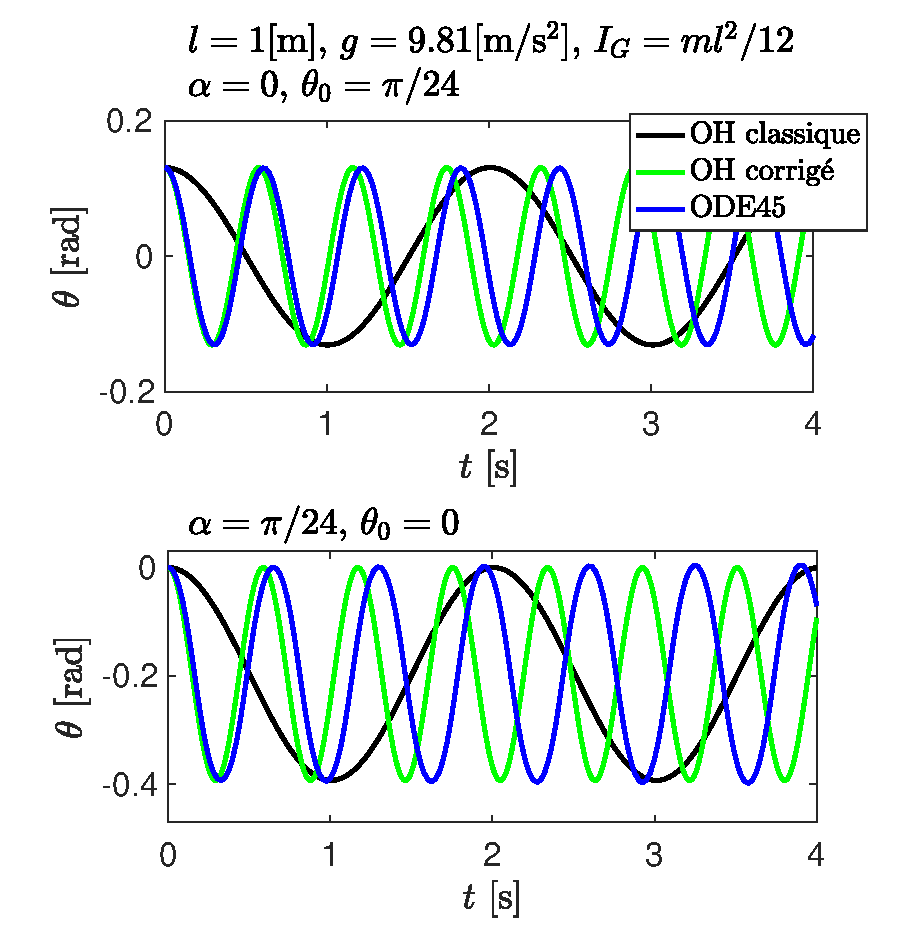
\includegraphics[width=0.95\linewidth]{ExoFig/tyr_solution_petites_oscillations.eps}
      \caption{Small oscillations around equilibrium.}
        \label{fig:solution_petites_oscillations}
    \end{subfigure}%
    \begin{subfigure}{.55\textwidth}
      \centering
        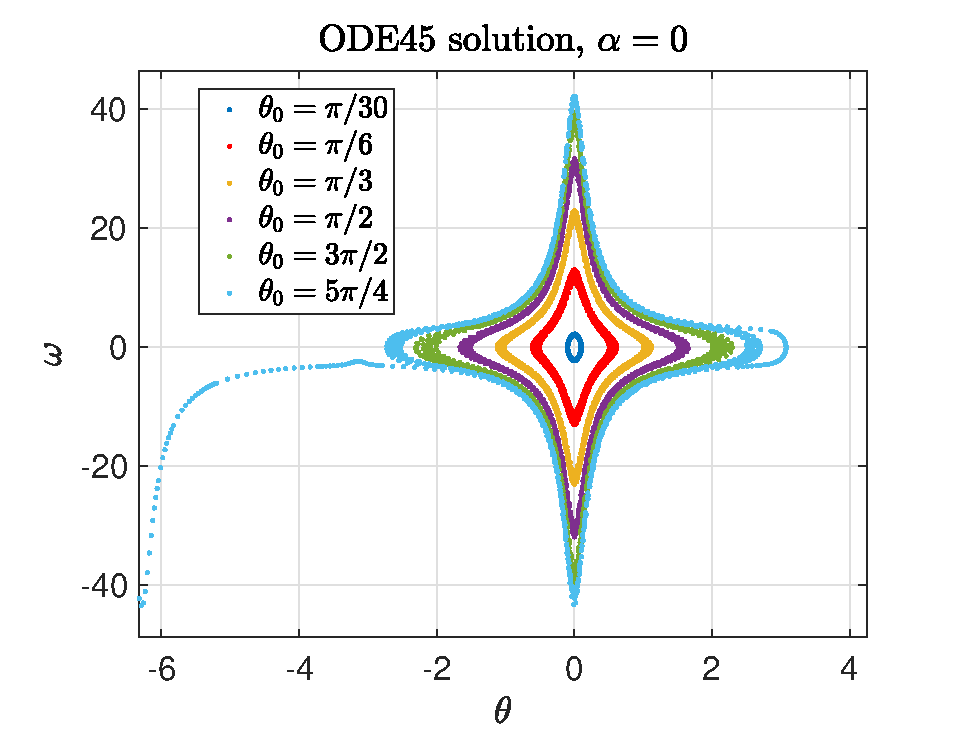
\includegraphics[width=0.95\linewidth]{ExoFig/tyr_solution_espace_de_phase.eps}
      \caption{Trajectories in phase space for different initial conditions.}
        \label{fig:espace_phase}
    \end{subfigure}
    \caption{Example of trajectories calculated by \texttt{tyrolienne.m} and ODE45.N.B.: these results use a $\theta$ defined with respect to the vertical and not with respect to the perpendicular of the cable, hence the oscillations around $\theta=-\alpha$.}
    \label{fig:test}
    \end{figure}
%\end{solution}


%% PART 2
\uplevel{We now consider the case $0<\alpha<\pi/2$. The zipline is released from point $O$, perpendicular to the cable and without initial velocity, i.e., at this moment, $\theta=0$, $\dot\theta=0$, and $\dot x_{A}=0$.}

\part{Find a relation that determines the maximum angle $\theta_{max}$ that the zipline reaches at the end of its course (when $x_A=d$) as a function of the problem data. 
Under what conditions does the zipline manage to perform complete rotations around point $B$?}
%\begin{solution}
    \par\vspace{2mm}
    We proceed using conservation laws between key moments.
    \subsubsection*{Moment $a$: initial condition}
    The mechanical energy at point $O$, moment $a$ ($t=t_0$), consists solely of potential energy, i.e.,
    \begin{equation}
        E_{a} =mgh
    \end{equation}
    with $h=d\sin\alpha$ (we keep the letter h until the end for simplicity). 
    Here, we set the zero of potential energy when the zipline is at point $B$ at $\theta=0$.
    
    \subsubsection*{Moment $b$: just before the impact}
    Just before reaching point $B$, moment $b$, the potential energy is zero, and the zipline does not rotate (equilibrium position).
    The mechanical energy is thus equal to the translational kinetic energy, i.e.,
    \begin{equation}
        E_{b} = \frac{1}{2}mv_{G,b}^2.
    \end{equation}
    Between moments $a$ and $b$, mechanical energy is conserved (only gravity works)
    \begin{equation}
        E_{a} = E_{b} \Leftrightarrow mgh = \frac{1}{2}mv_{G,b}^2,
    \end{equation}
    which gives the velocity of the center of mass (and the entire zipline by extension) upon reaching point $B$, $v_{G,b}=\sqrt{2gh}$.
    The angular momentum at point $A$ at moment $b$ is given by 
    \begin{equation}
        \bm L_{A,b} =\sum_i\overrightarrow{AP_i}\times m_i \bm v_{i,b} = \overrightarrow{AG}\times m \bm v_{G,b} + I_G \omega_b \ezACDH = ml\sqrt{2gh}\ezACDH,
    \end{equation}
    where $\omega_b=0$ because the bar does not perform proper rotation at this moment.
    
    \subsubsection*{Moment $c$: just after the impact}
    During the interaction with the mechanism at point $B$, the velocity of the attachment point changes from $\dot x_{A}\exACDH =v_{G,b}\exACDH$ to $\dot x_{A}\exACDH =0$.
    There is thus a non-zero acceleration of the attachment point, implying the existence of a force $F_B\exACDH$ by Newton's second law.
    This force works because it is parallel to the velocity of the point where it is applied.
    This is why neither mechanical energy nor momentum is conserved between moments $b$ and $c$.
    However, since the torque associated with $\vec F_B$ is zero ($\vec M_B=\overrightarrow{AB}\times\vec F_B = 0$ because $\overrightarrow{AB}=0$), the angular momentum at point $A$ is conserved during the impact.
    Thus, just after the impact, the angular momentum at point $A$ is expressed as
    \begin{equation}
        \bm L_{A,c} =\overrightarrow{AG}\times m \bm v_{G,c} + I_G \omega_c \ezACDH = (1+\eta)mlv_{G,c}\ezACDH
    \end{equation}
    where we used $v_{G,c} =  l\omega_c$.
    We now equate the angular momentum before and after the impact to obtain the velocity of the center of mass at moment $c$, i.e.,
    \begin{equation}
        \bm L_{A,c} = \bm L_{A,b} \Leftrightarrow (1+\eta)mlv_{G,c} = ml\sqrt{2gh} \Leftrightarrow v_{G,c}= \frac{\sqrt{2gh}}{1+\eta}.
        \label{eq:mcin_A_c}
    \end{equation}
    The mechanical energy at moment $c$ is given by
    \begin{equation}
    E_{c} = \frac{1}{2}mv_{G,c}^2 + \frac{1}{2}I_G\omega_c^2 = \frac{1}{2}m\left(v_{G,c}^2 + \frac{I_G}{ml^2}v_{G,c}^2\right) = (1+\eta)\frac{1}{2}m v_{G,c}^2.
    \end{equation}
    
    \noteACDH{We can verify that mechanical energy is not conserved by calculating its variation between moments $b$ and $c$
    $$
    E_{c} - E_{b} = (1+\eta)\frac{1}{2}m v_{G,c}^2 - \frac{1}{2}mv_{G,b}^2 =\left[(1+\eta) - (1+\eta)^2\right]\frac{1}{2}m v_{G,c}^2 = -\eta E_{c} = -\frac{\eta}{1+\eta}E_b < 0.
    $$
    Since $\eta>0$, we conclude that energy is absorbed by the mechanism.
    The relative energy variation is given by $\delta = |E_c-E_b|/E_b = \eta/(1+\eta)$. 
    For a homogeneous bar ($I_G = ml^2/48$), we obtain $\delta = 1/49$, whereas for a pendulum ($I_G=ml^2$), we have $\delta = 1/2$, i.e., $50\%$ of the initial energy is absorbed by the mechanism.}
    
    \subsubsection*{Moment d: maximum amplitude}
    When the maximum amplitude is reached, moment $d$, the zipline no longer rotates, $\omega_{d}=0$, so the mechanical energy is expressed as
    \begin{equation}
        E_{d} = mgh_{max}
    \end{equation}
    Mechanical energy is conserved between post-impact ($c$) and maximum amplitude ($d$), so we can obtain an equation for $\theta_{max}$ using $h_{max}=l \cos(\alpha)-l\cos(\theta_{max}-\alpha)$, i.e.,
    \begin{align}
        &(1+\eta)\frac{1}{2}mv_{G,c}^2 = mgh_{max} \nonumber\\
        \Leftrightarrow&\frac{mgh}{1+\eta} =mg l [\cos(\alpha)-\cos(\theta_{max}-\alpha)] \nonumber\\
        \Leftrightarrow&\cos(\theta_{max}-\alpha) = \cos(\alpha) - \frac{1}{1+\eta}\frac{h}{l}\nonumber\\
        \Leftrightarrow&\theta_{max}=\alpha+\arccos\left[\cos(\alpha) - \frac{1}{1+\eta}\frac{d}{l}\sin(\alpha)\right].
        \label{eq:ampmax}
    \end{align}
    Since $-1\leq \cos \leq 1$, Eq. \eqref{eq:ampmax} does not always have a solution.
    This is related to the fact that above a certain starting height, the bar will not stop and will continue to rotate indefinitely around point $B$ according to our model.
    The limiting angle is $\theta_{lim}=\alpha+\pi$, and thus the limiting distance is
    \begin{align}
        d_{lim} = (1+\eta) \frac{\cos(\alpha) + 1}{\sin(\alpha)}l
        \label{eq:hlim}
    \end{align}
    And so the bar will perform rotations on itself if $d>d_{lim}$.
    
    
    \noteACDH{Let us study some limits to convince ourselves of the result.
    If $\alpha=2n\pi$, $\sin\alpha=0$ and $\cos\alpha=1$, and thus $d_{lim}=\infty$, which is logical because we are in the case of a horizontal cable, and complete rotations are not possible with a zero starting angle.
    If $\alpha=(2n+1)\pi$, $\sin\alpha=0$ and $\cos\alpha=-1$, and thus $d_{lim}="0/0"$.
    We calculate this limit using L'Hospital's theorem and obtain $d_{lim}=0$, which is logical because we are in the "flipped" case where the zipline is above the cable.
    For $\alpha =\pi/2$, we have $d_{lim}=(1+\eta)l$, which gives $d_{lim}=2l$ in the case of a pendulum ($\eta = 1$). 
    This result coincides with the result on the $\delta$ of mechanical energy absorbed by the mechanism, which predicted a loss of $50\%$ of initial energy. }
%\end{solution}

\end{parts}
\end{document}